\documentclass[a4paper,11pt,twoside]{memoir}
\chapterstyle{veelo}

\usepackage{TUINFDA}

\usepackage{url}
\usepackage{hyperref}					% links in pdf
\usepackage{graphicx}            			% Figures
\usepackage{verbatim}            			% Code-Environment
\usepackage[lined,linesnumbered,algochapter]{algorithm2e} % Algorithm-Environment

\usepackage{pgf}					
\usepackage{tikz}					% tikz graphics
\usetikzlibrary{arrows,automata}

\usepackage{ngerman}
\usepackage[ngerman]{babel}
\usepackage{bibgerm,cite}       % Deutsche Bezeichnungen, Automatisches Zusammenfassen von Literaturstellen
\usepackage[ngerman]{varioref}  % Querverweise
% to use the german charset include cp850 for MS-DOS, ansinew for Windows and latin1 for Linux.
% \usepackage[latin1]{inputenc}

\thesistitle{Digital Audio Watermarking}
\thesissubtitle{f\"ur analoge \"Ubertragungsstrecken} % optional
\thesisdate{\today}

% all titles and designations have to be gender-related!
%\thesisdegree{Bachelor of Science}
%\thesiscurriculum{Medieninformatik und Visual Computing} % your study
\thesisverfassung{Maximilian Irro} % Verfasser
\thesisauthor{Maximilian Irro} % your name
\thesisauthoraddress{Pfalzstra{\ss}e 10, 5282 Ranshofen} % your address
\thesismatrikelno{1026859} % your registration number

\thesistype{Bachelorarbeit aus Informatik}

\thesisbetreins{Dipl.-Ing. Mag. Dr. Matthias Zeppelzauer}
%\thesisbetrzwei{Dr. Vorname Familienname}
%\thesisbetrdrei{Dr. Vorname Familienname} % optional

% define page numbering styles
\makepagestyle{numberCorner}
\makeevenfoot{numberCorner}{\thepage}{}{}
\makeoddfoot{numberCorner}{}{}{\thepage}

% define custom macros for specific formats or names
\newcommand{\uml}[1]{\texttt{#1}}
\newcommand{\cd}{\textsf{Class Diagram}}

% define newline hight between two paragraphs - by default there is none
\setlength{\parskip}{0.15in}

\begin{document}

\captionnamefont{\bfseries}

%%%%%%%%%%%%%%%%%%%%%%%%%%%%%%%%%%%%%%%%%
%%%   FRONTMATTER    %%%%%%%%%%%%%%%%%%%%
%%%%%%%%%%%%%%%%%%%%%%%%%%%%%%%%%%%%%%%%%
\frontmatter
\pagenumbering{roman}

%%%%%%%%%%%%%%%%%%%%%%%%%%%%%%%%%%%%%%%%%
%%%   TITLEPAGES    %%%%%%%%%%%%%%%%%%%%%
%%%%%%%%%%%%%%%%%%%%%%%%%%%%%%%%%%%%%%%%%

% the german title page is required as first page
% $Id: titlepage.tex 1752 2010-03-20 11:07:02Z tkren $
%
% TU Wien - Faculty of Informatics
% thesis titlepage
%
% This titlepage is using the geometry package, see
% <http://www.ctan.org/macros/latex/contrib/geometry/geometry.pdf>
%
% For questions and comments send an email to
% Thomas Krennwallner <tkren@kr.tuwien.ac.at>
% or to Petra Brosch <brosch@big.tuwien.ac.at>
%

\selectlanguage{ngerman}

% setup page dimensions for titlepage
\newgeometry{left=2.4cm,right=2.4cm,bottom=2.5cm,top=2cm}

% force baselineskip and parindent
\newlength{\tmpbaselineskip}
\setlength{\tmpbaselineskip}{\baselineskip}
\setlength{\baselineskip}{13.6pt}
\newlength{\tmpparindent}
\setlength{\tmpparindent}{\parindent}
\setlength{\parindent}{17pt}

% first titlepage
\thispagestyle{tuinftitlepage}

%
% Kludge: for each titlepage set \pagenumbering to a different
% style. This is used to fix a problem with hyperref, because there
% are multiple "page 1" and hyperref hates that
%
\pagenumbering{Alph}

\begin{center}
{\ \vspace{3.4cm}}

\begin{minipage}[t][2.8cm][s]{\textwidth}%
\centering
\thesistitlefontHUGE\sffamily\bfseries\tuinfthesistitle\\
\bigskip
{\thesistitlefonthuge\sffamily\bfseries\tuinfthesissubtitle}
\end{minipage}

\vspace{1.3cm}

{\thesistitlefontLARGE\sffamily \tuinfthesistype}

\vspace{6mm}

%{\thesistitlefontlarge\sffamily zur Erlangung des akademischen Grades}
%
%\vspace{6mm}
%
%{\thesistitlefontLARGE\sffamily\bfseries \tuinfthesisdegree}
%
%\vspace{6mm}
%
%{\thesistitlefontlarge\sffamily im Rahmen des Studiums}
%
%\vspace{6mm}
%
%{\thesistitlefontLarge\sffamily\bfseries \tuinfthesiscurriculum}
%
%\vspace{6.5mm}

{\thesistitlefontlarge\sffamily von}

\vspace{6mm}

{\thesistitlefontLarge\sffamily\bfseries \tuinfthesisauthor}

\vspace{1.5mm}

{\thesistitlefontlarge\sffamily Matrikelnummer \tuinfthesismatrikelno} 

\vspace{3cm} %default: 1.4cm



\begin{minipage}[t][4cm][t]{\textwidth}%
  \vspace{0pt}\raggedright\thesistitlefontnormalsize\sffamily
  %
  \centering
  
  unter der Betreuung von 
  
  \tuinfthesisbetreins
  
%  \begin{tabbing}%
%	    \hspace{19mm} \= \hspace{66mm} \kill
%	    betreut von \> \tuinfthesisbetreins\\
%%	    Mitwirkung: \> \tuinfthesisbetrzwei\\
%%	                \> \tuinfthesisbetrdrei
%  \end{tabbing}
\end{minipage}

\vspace{0pt}\raggedright\thesistitlefontnormalsize\sffamily
\begin{minipage}[t][1.6cm][t]{\textwidth}%
  %
  \centering

  Interactive Media Systems Group

  Institut f\"ur Softwaretechnik und Interaktive Systeme

  Fakult\"{a}t f\"{u}r Informatik 

  Technische Universit\"{a}t Wien

\end{minipage}



%\begin{minipage}[t][1.5cm][t]{\textwidth}%
%  \vspace{0pt}\sffamily\thesistitlefontnormalsize
%  \begin{tabbing}%
%    \hspace{45mm} \= \hspace{63mm} \= \hspace{51mm} \kill
%    Wien, \tuinfthesisdate \> {\raggedright\rule{51mm}{0.5pt}} \> {\raggedright\rule{51mm}{0.5pt}} \\
%    \> \begin{minipage}[t][0.5cm][t]{51mm}\centering (Unterschrift \tuinfthesisverfassung)\end{minipage}
%    \> \begin{minipage}[t][0.5cm][t]{51mm}\centering (Unterschrift \tuinfthesisbetreuung)\end{minipage}
%    \end{tabbing}
%\end{minipage}

\end{center}

% we want an empty page right after first titlepage
\pagestyle{empty}
\cleardoublepage

% we're done with the titlepages, proceed with default pagenumbering
\pagenumbering{roman}

% restore baselineskip
\setlength{\baselineskip}{\tmpbaselineskip}
\setlength{\parindent}{\tmpparindent}

% back to normal geometry
\restoregeometry

\selectlanguage{english}

%%% Local Variables:
%%% TeX-PDF-mode: t
%%% TeX-debug-bad-boxes: t
%%% TeX-parse-self: t
%%% TeX-auto-save: t
%%% reftex-plug-into-AUCTeX: t
%%% End:


% an english translation may follow
%% $Id: titlepage.tex 1752 2010-03-20 11:07:02Z tkren $
%
% TU Wien - Faculty of Informatics
% thesis titlepage
%
% This titlepage is using the geometry package, see
% <http://www.ctan.org/macros/latex/contrib/geometry/geometry.pdf>
%
% For questions and comments send an email to
% Thomas Krennwallner <tkren@kr.tuwien.ac.at>
% or to Petra Brosch <brosch@big.tuwien.ac.at>
%

% setup page dimensions for titlepage
\newgeometry{left=2.4cm,right=2.4cm,bottom=2.5cm,top=2cm}

% force baselineskip and parindent
%\newlength{\tmpbaselineskip}
%\setlength{\tmpbaselineskip}{\baselineskip}
%\setlength{\baselineskip}{13.6pt}
%\newlength{\tmpparindent}
%\setlength{\tmpparindent}{\parindent}
%\setlength{\parindent}{17pt}

% first titlepage
\thispagestyle{tuinftitlepage}

%
% Kludge: for each titlepage set \pagenumbering to a different
% style. This is used to fix a problem with hyperref, because there
% are multiple "page 1" and hyperref hates that
%
\pagenumbering{Roman}

\begin{center}
{\ \vspace{3.4cm}}

\begin{minipage}[t][2.8cm][s]{\textwidth}%
\centering
\thesistitlefontHUGE\sffamily\bfseries\tuinfthesistitle\\
\bigskip
{\thesistitlefonthuge\sffamily\bfseries\tuinfthesissubtitle}
\end{minipage}

\vspace{1.3cm}

{\thesistitlefontLARGE\sffamily \tuinfthesistypeen}

\vspace{6mm}

{\thesistitlefontlarge\sffamily submitted in partial fulfillment of the requirements for the degree of}

\vspace{6mm}

{\thesistitlefontLARGE\sffamily\bfseries \tuinfthesisdegreeen}

\vspace{6mm}

{\thesistitlefontlarge\sffamily in}

\vspace{6mm}

{\thesistitlefontLarge\sffamily\bfseries \tuinfthesiscurriculumen}

\vspace{6.5mm}

{\thesistitlefontlarge\sffamily by}

\vspace{6mm}

{\thesistitlefontLarge\sffamily\bfseries \tuinfthesisauthor}

\vspace{1.5mm}

{\thesistitlefontlarge\sffamily Registration Number \tuinfthesismatrikelno} 

\vspace{1.4cm}

\begin{minipage}[t][1.6cm][t]{\textwidth}%
  \vspace{0pt}\raggedright\thesistitlefontnormalsize\sffamily
  %
  to the Faculty of Informatics 

  at the Vienna University of Technology
\end{minipage}

\vspace{0pt}\raggedright\thesistitlefontnormalsize\sffamily
\begin{minipage}[t][4cm][t]{\textwidth}%
  \begin{tabbing}%
	    \hspace{19mm} \= \hspace{66mm} \kill
	    Advisor: \> \tuinfthesisbetreins\\
	    Assistance: \> \tuinfthesisbetrzwei\\
	                \> \tuinfthesisbetrdrei
     \end{tabbing}
\end{minipage}

\begin{minipage}[t][1.5cm][t]{\textwidth}%
  \vspace{0pt}\sffamily\thesistitlefontnormalsize
  \begin{tabbing}%
    \hspace{45mm} \= \hspace{63mm} \= \hspace{51mm} \kill
    Vienna, \tuinfthesisdate \> {\raggedright\rule{51mm}{0.5pt}} \> {\raggedright\rule{51mm}{0.5pt}} \\
    \> \begin{minipage}[t][0.5cm][t]{51mm}\centering (Signature of Author)\end{minipage}
    \> \begin{minipage}[t][0.5cm][t]{51mm}\centering (Signature of Advisor)\end{minipage}
    \end{tabbing}
\end{minipage}

\end{center}

% we want an empty page right after first titlepage
\pagestyle{empty}
\cleardoublepage

% we're done with the titlepages, proceed with default pagenumbering
\pagenumbering{roman}

% restore baselineskip
\setlength{\baselineskip}{\tmpbaselineskip}
\setlength{\parindent}{\tmpparindent}

% back to normal geometry
\restoregeometry


%%% Local Variables:
%%% TeX-PDF-mode: t
%%% TeX-debug-bad-boxes: t
%%% TeX-parse-self: t
%%% TeX-auto-save: t
%%% reftex-plug-into-AUCTeX: t
%%% End:
 % optional

%%%%%%%%%%%%%%%%%%%%%%%%%%%%%%%%%%%%%%%%%
%%%   ERKLAERUNG DER SELBSTAENDIGKEIT   %
%%%%%%%%%%%%%%%%%%%%%%%%%%%%%%%%%%%%%%%%%
\cleardoublepage
\selectlanguage{ngerman}
\chapter*{Erklärung zur Verfassung der Arbeit}

\tuinfthesisauthor\\
\tuinfthesisauthoraddress

\vspace*{1.2cm}

Hiermit erkläre ich, dass ich diese Arbeit selbständig verfasst habe, 
dass ich die verwendeten Quellen und Hilfsmittel vollständig angegeben 
habe und dass ich die Stellen der Arbeit - einschließlich Tabellen, 
Karten und Abbildungen -, die anderen Werken oder dem Internet im 
Wortlaut oder dem Sinn nach entnommen sind, auf jeden Fall unter Angabe 
der Quelle als Entlehnung kenntlich gemacht habe.\\

\vspace*{2cm}
\begin{tabbing}%
    \hspace{58mm} \= \hspace{28mm} \= \hspace{58mm} \kill
    {\raggedright\rule{58mm}{0.5pt}} \> \> {\raggedright\rule{58mm}{0.5pt}} \\
    \begin{minipage}[t][0.5cm][t]{58mm}
	\vspace{0pt}\sffamily\thesistitlefontnormalsize
	\centering (Ort, Datum)
    \end{minipage}
    \> \>
    \begin{minipage}[t][0.5cm][t]{58mm}
	\vspace{0pt}\sffamily\thesistitlefontnormalsize
	\centering (Unterschrift \tuinfthesisverfassung)
    \end{minipage}
\end{tabbing}


\selectlanguage{english}

%%%%%%%%%%%%%%%%%%%%%%%%%%%%%%%%%%%%%%%%%
%%%   ACKNOWLEDGEMENTS    %%%%%%%%%%%%%%%
%%%%%%%%%%%%%%%%%%%%%%%%%%%%%%%%%%%%%%%%%

% optional acknowledgements may be included in german or in english
%\chapter*{Danksagung}

Es gilt einigen Personen zu danken:

Meinem Betreuer Matthias Zeppelzauer, unter dessen Anleitung diese Arbeit entstanden ist.

J\"urgen K\"ochl, der sich mehrmals die Zeit stehlen lie{\ss} um sich mit mir den Freuden der Fehlerkorrektur in der Signalverarbeitung hinzugeben.

John-Paul \glqq hukl\grqq{} Bader, der mit seinen Betr\"agen zu analogem und digitalem Audio im Podcast \emph{Freakshow}\footnote{\url{http://freakshow.fm}} mehr als einmal an einer Inspiration Schuld tr\"agt. 

Shijun Xiang, der mich durch seine typografischen Ausrutscher zeitweilens l\"anger wach hielt und somit sicherstellte, dass ich mich keiner ansonsten wom\"oglich ungesund gro{\ss}en Menge Schlaf hingebe. 
 		% optional
\chapter*{Acknowledgements}

Optional acknowledgements may be inserted here.	% optional

%%%%%%%%%%%%%%%%%%%%%%%%%%%%%%%%%%%%%%%%%
%%%   ABSTARCT    %%%%%%%%%%%%%%%%%%%%%%%
%%%%%%%%%%%%%%%%%%%%%%%%%%%%%%%%%%%%%%%%%

\chapter*{Abstract}

While digital audio watermarking is already a widespread practice, most research only concern copyright protection mechanisms. An aim on open information integration is hardly ever a focus of development goals. Yet there are use cases were additional information in audio signals would be of most value. Especially digital/analog (DA) conversion processes\index{DA-Wandlung} tend to lose all sorts of metadata, for them not being translated into acoustic signals.
This is where watermarks may come to aid. Also they could be utilized to add additional information to radio and TV broadcast which would make them accessible not only to the receiving device.

This paper describes the implementations of an existing watermarking algorithm claiming to be capable of enduring DA conversions. Additionally a framework is proposed to utilize the algorithm in a developed communication protocol with synchronization-codes and error-correction mechanisms to provide a well defined, stable communication channel.


\cleardoublepage
\selectlanguage{ngerman}
\chapter*{Kurzfassung}

Hier fügen Sie die Kurzfassung auf Deutsch gemäß den Vorgaben der Fakultät ein.

\selectlanguage{english}

%%%%%%%%%%%%%%%%%%%%%%%%%%%%%%%%%%%%%%%%%
%%%   CONTENTS    %%%%%%%%%%%%%%%%%%%%%%%
%%%%%%%%%%%%%%%%%%%%%%%%%%%%%%%%%%%%%%%%%
% uncomment to set document language to german (results in "Inhaltsverzeichnis", "Kapitel", "Abbildung", etc. instead of "Contents", "Chapter", and "Figure"), otherwise the document's language is english
\selectlanguage{ngerman}

\setcounter{tocdepth}{3}
\setcounter{secnumdepth}{3}

\cleardoublepage
\pagestyle{numberCorner}
\tableofcontents*

%%%%%%%%%%%%%%%%%%%%%%%%%%%%%%%%%%%%%%%%%
%%%   MAINMATTER    %%%%%%%%%%%%%%%%%%%%%
%%%%%%%%%%%%%%%%%%%%%%%%%%%%%%%%%%%%%%%%%

\mainmatter
\pagenumbering{arabic}
\pagestyle{numberCorner}

%%%%%%%%%%%%%%%%%%%%%%%%%%%%%%%%%%%%%%%%%
\chapter{Einf\"uhrung}
\label{ch:intro}

\section{Motivation}

Die Digitalisierung unserer Welt schreitet seit mehr als 50 Jahren stetig voran. Immer mehr liegt nur mehr in digitaler Form vor. Und durch die wachsende Vernetzung stehen diese Daten vor allem seit dem neuen Jahrtausend immer mehr Menschen mit immer weniger Aufwand jederzeit zur Verfügung. 

Doch es ergibt sich daraus auch ein Problem: \textit{Was liegt eigentlich vor?} Digitale (und vor allem multimediale) Daten sagen per se nichts über ihre Bedeutung aus. Sie bekommen diese durch den Betrachter. Doch aus diversen Gründen, ganz voran alleine um sie sortieren und suchen zu können, ist es aber interessant ihnen bereits vorher eine gewisse Bedeutung zuzuschreiben. Dadurch wurde in den letzten Jahren ein Stichwort groß: \textit{Metadaten}\index{Metadaten}. Metadaten sind \glqq{}Daten über Daten\grqq{}. Mit ihnen wird versucht vorliegende Daten zu beschreiben (z.B. Genre eines Musikstücks), zusätzliche Informationen über sie vorzuhalten (Künstler und Album eines Musikstücks), diese maschinenlesbar bereitzustellen (ID3-Tags bei MP3) und wenn möglich auch direkt mit den Daten zu verknüpfen (Kapitelmarken in MP4/M4B Hörbüchern).

Das Problem bei Metadaten ist sie bereitzustellen und vorzuhalten. Seit dem Ausbau der digitalen Vernetzung liegen Metadaten oft nicht mehr direkt bei den eigentlichen Daten. Oftmals sind sie auf einem externen Server und werden bei Bedarf angefordert. Die Metadaten sind nur dann zugänglich, wenn der Server verfügbar ist und ein Mechanismus existiert mit dem die Daten eindeutig mit den Metadaten am Server verknüpft werden können. 
Eine Datei kann auch durch eine zusätzliche standardisierte Datei im selben Namespace beschrieben werden (etwa via XML). Kopiert man jedoch nur die ursprünglichen Daten, nicht aber ihre Metadaten, so geht die zusätzliche Information verloren. 

Es ist daher oftmals wünschenswert die Metadaten direkt \textit{in} den eigentlichen Daten vorzuhalten. Eine der vielleicht bekanntesten Formen dieser Art der Metadatenspeicherung sind die bereits oben erwähnten MP3 Tags. Hier werden die Metadaten einfach am Ende des Audiosignals angehängt. Diese Form der Metadatenspeicherung ist vor allem bei digitalen, multimedialen Daten besonders beliebt. Nicht zuletzt die MPEG\footnote{Moving Picture Experts Group. Eine Vereinigung zur Standardisierung von Audio- und Video-Kompressionsalgorithmen und Containerformaten. Am bekanntesten dürfte das MP4 Dateiformat sein.} treibt diese Entwicklung mit ihren Standards auch rege voran. 

\section{Digital und analoge Daten}

Bei digitalen Daten lassen sich die Metadaten oftmals noch recht einfach direkt zu den eigentlichen Daten speichern. Es muss nur einen entsprechenden Standard geben wie diese an die Daten angehängt werden können. Doch vor allem multimediale Daten existieren in der Regel nicht nur in digitaler Form. Spätestens wenn sie konsumiert (betrachtet, gehört) werden sollen müssen sie auf die eine oder andere Art in eine analoge Form gebracht werden. Dabei gehen die Metadaten meistens verloren. Dem wird entgegen gesetzt, dass die Metadaten meistens an diesem Punkt auch angezeigt werden. Die meisten MP3 Player zeigen während des Abspielens den Tracktitel und Artist an. Allerdings ist der Lifecycle der Metadaten an dieser Stelle auch beendet. Werden die nun analogen Daten weiter aufgezeichnet, verarbeitet und verwendet, so ist ihre Beschreibung verloren gegangen, wenn sich nicht jemand explizit \glqq{}von Hand\grqq{} darum weiterträgt. Es wäre also Wünschenswert wenn die Metadaten auch im analogen Zustand Teil der Daten wären. 

\section{Digitale Wasserzeichen}

Digitale Wasserzeichen (engl. \textit{Digital Watermarks}) sind sämtliche Verfahren die ein digitales Signal (Audio, Video, aber auch nur einfache Bilder) so verändern, dass in ihm ein weiteres Signal versteckt ist. Da dieses zusätzliche Signal in der Regel unwahrnehmbar ist (oder zumindest sein soll) ist die Einbettung dieses \glqq{}versteckten Signals\grqq{} in der ursprüngliche (das \glqq{}Trägersignal\grqq{}) also eine steganographische Methode.
Somit kann beispielsweise ein Bild in einem anderen Bild versteckt werden. Zu beachten ist natürlich, dass die Einbettungskapazität durchaus limitiert ist, da die Qualität des Trägersignal nicht maßgeblich beeinträchtigt werden soll. 

Prinzipiell lassen sich Watermarks in 2 Kategorien unterteilen\cite{arnold2000audio}: 

\begin{description}
	
	\item[Secret watermarks] sollen unauffindbar, außer für jene die dazu berechtigt sind. Sie stellen einen gesicherten Übertragungskanal zwischen den autorisierten Personen dar, die zu den versteckten Informationen durch ihr Wissen um ein geheimes Verfahren oder einen geheimen Schlüssel Zugang haben. Die Existenz des Watermarks an sich sollte nach Möglichkeit für Unautorisierte nicht nachweisbar sein. 
	
	\item[Public watermarks] sollen für jeden unter Anwendung des Dekodierungsverfahrens lesbar sein. Sie sind somit ein öffentlicher Übertragungskanal, da das Verfahren transparent gestaltet ist.
	
\end{description}

\section{Anwendungsgebiete}

Digitale Wasserzeichen erfreuen sich zunehmender Beliebtheit seitdem es möglich ist praktisch kostenlos perfekte digitale Kopien von Audio, Video, Bildern und Texten herzustellen\cite{mintzer1997effective}. Indem in mediale Daten Wasserzeichen eingebracht werden, wird Urheberschaft kenntlich gemacht und Copyrightanliegen können verfolgt werden. In Bildern wird ein Wasserzeichen eingebracht, das nicht sichtbar ist, trotzdem bei Bedarf aus dem Bild eindeutig extrahiert werden kann. Somit kann überprüft werden, ob Bilder unlizenziert Verwendung finden. In Musikdateien ermöglichen individuelle Wasserzeichen zu jedem Track den ursprünglichen Käufer ausfindig zu machen, seitdem es Dank des MP3-Komprimierungsverfahrens möglich geworden ist Musikdateien in geringer Datengröße und dennoch guter Qualität problemlos (und oftmals illegal) durch das Internet zu kopieren. Bei Videodaten kann festgestellt werden, ob diese nachträglich verändert wurden (bei Beweisaufnahmen etwa). 

In den Anfangszeiten der digitalen Wasserzeichen wurden auch Überlegungen angestellt wie die aufkommenden DVDs so gekennzeichnet werden könnten, dass eine Kopierung nur im Rahmen des erlaubten Copyrights stattfindet\cite{petitcolas1999information}. Die Idee war alle DVD Player so zu Programmieren, dass sie keine Kopien von kommerziellen Inhalten anfertigen. TV-Ausstrahlungen würden hingegen so gekennzeichnet, dass sie genau einmal kopiert werden könnten und private Aufnahmen wären unlimitiert kopierbar. 

\section{Ziele}

In dieser Arbeit wird versucht ein transparentes Watermarkingverfahren für digitale Audiosignale umzusetzen, welches die Übertragung über eine analoge Übertragungsstrecke (etwa Luft) übersteht. Damit könnten Metadaten direkt in Audiosignalen untergebracht und erhalten werden, auch wenn sie über ein Lautsprechersystem abgespielt werden. Entsprechende Empfangsgerät (z.B. ein Handy) könnten dann das Signal aufnehmen und die darin enthaltenen Daten wieder rekonstruieren. Ein denkbarer Anwendungsfall wären etwa die Metadaten der Musiktracks im Programm eines Radiosenders.

Watermarkingverfahren zum Urheberrechtsschutz sind im aktuellen Stand der Technik bereits weit ausgereift. Hingegen wurde bisher nur wenig Augenmerkt auf die Resistenz bei DA/AD Wandlung gelegt, da dies zur Beseitigung der Copyright-Watermarks kaum ein angewandter Angriffsvektor ist. Die Auswirkungen auf die resultierende Qualität sind in der Regel zu massiv. 

Diese Arbeit stützt sich vor allem auf das von Shijun Xiang\cite{xiang2007robust} vorgeschlagene Audio-Watermarkingverfahren für D/A-A/D Wandlung\index{D/A-A/D Wandlung}. Dokumentiert ist hier die Implementierung dieser sowie deren Erweiterungen und Modifikationen. 



%%%%%%%%%%%%%%%%%%%%%%%%%%%%%%%%%%%%%%%%%
%%%%%%%%%%%%%%%%%%%%%%%%%%%%%%%%%%%%%%%%%
%%%    THEORETISCHE GRUNDLAGEN    %%%%%%%
%%%%%%%%%%%%%%%%%%%%%%%%%%%%%%%%%%%%%%%%%

\section{Allgemein}

Hier werden die mathematischen Grundlagen beschrieben. Ich plane mich hier vor allem auf das Prinzip der Einbettung von 0en und 1en zu konzentrieren. 

\section{Einbettungsstrategie}


\section{Diskrete Wavelet Transformation}

%%%%%%%%%%%%%%%%%%%%%%%%%%%%%%%%%%%%%%%%%
\chapter{Implementierung}
\label{ch:methode}

In Kapitel \ref{ch:theorie} wurde das theoretisch-mathematische Modell beschrieben, mit welchem ein Bit geschrieben und wieder rekonstruiert werden kann. Um dieses Wissen nun praktisch nutzen zu können wurde ein Framework ausgearbeitet in dem es zur Anwendung kommt. 

\section{Architektur}

Das von Shannon und Weaver entwickelte Sender-Empfänger-Modell \cite{shannon2001mathematical} kann herangezogen werden, um den Aufbau des Kommunikationssystems zu modellieren:

\begin{figure}[h]
	\centering
	%\includesvg[width=0.7\textwidth]{figures/diagram-framework.svg}
	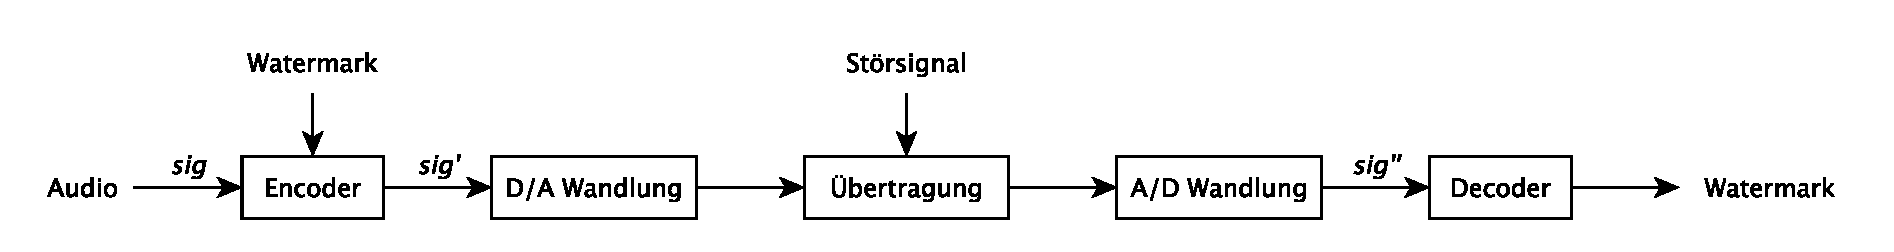
\includegraphics[width=0.9\textwidth]{figures/diagram-framework.pdf}
	\caption{Das Framework im Kommunikationsprozess}
	\label{fig:diagram-framework}
\end{figure}

Ein beliebiges digitales Signal soll mit einer Information, dem \textit{Watermark}\index{Watermark}, angereichert werden. Das Encodermodul verflechtet basierend auf der Grundlage von Kapitel \ref{sec:embeddingstragety_bitsequence} das Watermark mit dem Signal und liefert erneut ein digitales Signal.

Wir das neue digitale Signal auf analoger Ebene übertragen, muss eine DA-Wandlung\index{DA-Wandlung} vorgenommen werden. In der Regel wird das Signal über ein Lautsprechersystem abgespielt werden. Allerdings ist auch die reine Übertragung von einer Soundkarte zu einer anderen via einem Audiokabel eine DA-Wandlung. Ebenso würde das Pressen einer Schallplatte oder das Übertragen auf ein analoges Tonband in diese Kategorie fallen. 

Jede analoge Übertragung geschieht auf einem analogen Trägermedium, da Schall nicht im leeren Raum existieren kann, sondern sich auf einem Medium ausbreiten muss. Für den menschlichen Hörapparat ist dies normalerweise die Luft. Aber auch in Wasser kann sich Schall ausbreiten\footnote{Hier sogar viel besser. Viele Meereslebewesen nutzen diesen Umstand sehr stark aus, da sich Licht unter Wasser nur wenige 100 Meter ausbreitet. Auch das Sonar basiert darauf.} sowie in Festkörpern. In letzteren liegt oftmals das Signal nicht direkt als Schallwelle vor, sondern im Falle eines Audiokabels etwa als elektrisches Signal. 

Doch egal welches Medium benutzt wird, jeder Übertragungskanal\index{\"Ubertragungskanal} verändert das Signal durch seine Umwelteinflüsse während es ihn durchläuft. In der Luft etwa kommen die übrigen Geräusche der Umgebung hinzu, u.a. auch die Eigenreflexion der Schallwelle an der Umgebung. 
Wir wollen uns mit den diversen Formen und Ursachen von Störsignalen nicht näher befassen. Für uns ist wichtig, dass jede Störung das Signal verändert. Das mit Informationen angereicherte, modifizierte Signal überlagert sich also mit den Störungen. Dies wird sich in der Regel negativ auf das Watermark\index{Watermark} auswirken. 

Um das Watermark rekonstruieren zu können, muss das Signal zuerst wieder in eine digitale Form gebracht werden. Dies geschieht durch eine AD-Wandlung\index{AD-Wandlung}. Eine Schallwelle wird durch ein Mikrofon aufgenommen, ein elektrisches Signal durch den Line-in Eingang einer Soundkarte umgewandelt. 

Das Decodermodul versucht anschließend, das Watermark\index{Watermark} zu rekonstruieren. Hier gilt es zwei Probleme zu überwinden. Erstens muss das Watermark erkannt werden, d.h. der Decoder muss herausfinden wo eingebettete Daten sind. Dazu werden wir sog. \textit{Synchronisations-Codes} mit speziellen Eigenschaften bemühen (näheres in Abschnitt \ref{sec:barker-code}). Und zweitens müssen die eingeflochtenen Bits wieder \textit{richtig} rekonstruiert werden. Aufgrund des Störsignals welches im Übertragungskanal\index{\"Ubertragungskanal} das Signal in Mitleidenschaft zieht kann sich dies durchaus als schwierig herausstellen. Zur Erhöhung der Resistenz werden in Abschnitt \ref{sec:errorcorrection} Fehlerkorrekturverfahren\index{Fehlerkorrekturverfahren} eingeführt. Es sei allerdings an dieser Stelle bereits darauf hingewiesen, dass das Signal im Allgemeinen so weit deformiert werden kann, dass auch die Fehlerkorrektur eine sowohl vollständige wie auch richtige Rekonstruktion nicht gewährleisten kann. 

\section{Watermark Implantierung}
\label{sec:embedding}
\index{Watermark}

Der Implantationsprozess wird schematisch in Abbildung \ref{fig:diagram-encoder} modelliert. Ein anzureicherndes digitales Audiosignal wird zunächst in gleich große Bereiche segmentiert, d.h. die Samples des Signals werden in Gruppen zu je $N_s$\index{Sample-Section-Length} Samples zerteilt. In jede Gruppe (sog. \textit{Sample Section}\index{Sample Section}) wird genau 1 Bit kodiert. Der Einbettungsprozess geschieht in der DWT-Domain, daher werden die DWT-Koeffizienten \index{DWT-Koeffizienten} der Sample Section berechnet (eine Samples Section besteht aus einer Reihen aufeinander folgender Messpunkte eines Signal - sie beschreiben also einen Teil eines Signal und können ganz einfach wieder als eigenständiges Signal betrachtet werden). 

\begin{figure}[h]
	\centering
	%\includesvg[width=0.7\textwidth]{figures/diagram-framework.svg}
	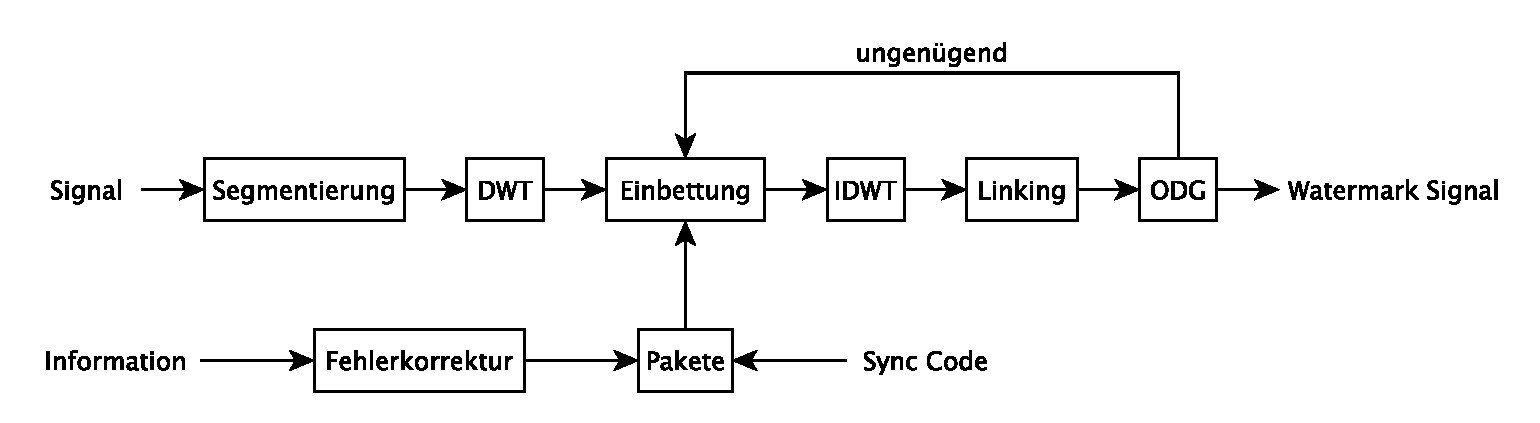
\includegraphics[width=\textwidth]{figures/diagram-encoder-v2.pdf}
	\caption{Schematischer Aufbau des Implemetierungsprozesses}
	\label{fig:diagram-encoder}
\end{figure}

Jede Sample Section\index{Sample Section} bekommt ein Bit der Bitsequenz, die das Signal beherbergen soll. Diese Sequenz setzt sich zusammen aus einer Kombination der mit Redundanz angereicherten (Abschnitt \ref{sec:errorcorrection}) eigentlichen Informationen und der Synchronisation-Codes\index{Synchronisations-Code}. Die Einbettung jedes Bit geschieht nach dem in Abschnitt \ref{sec:embeddingstragety} beschriebenen Algorithmus durch Veränderung der DWT-Koeffizienten\index{DWT-Koeffizienten}. Um das neue angereicherte Signal nun herzustellen werden auf die DWT-Koeffizienten eine inverse DWT-Transformation (IDWT)\index{inverse DWT-Transformation} angewandt. Diese resultiert in einer neuen Samples Section. Diese ersetzen im neuen Signal die unimplantierten Samples der korrelierenden Sample Section. 

Um sicherzustellen, dass das Watermark\index{Watermark} unhörbar in die Sample Section\index{Sample Section} implantiert wurde, wird noch eine Qualitätskontrolle vorgenommen. Dazu wird für ein Signalstück der sog. \textit{Objective Difference Grade} (ODG) berechnet. Erfüllt dieser einen vorgegebenen Grenzwert, so ist das Signal zu störhaft verändert worden und das Bit muss neu implantiert werden. Um eine weniger invasive Veränderung sicherzustellen wird der in Formel \ref{equ:embeddingstrength} eingeführte \textit{Embedding Strength Factor} (esf)\index{Embedding Strength Factor} reduziert, was dazu führt, dass die DWT-Koeffizienten weniger stark verändert werden.

\subsection{Synchronisations-Codes}
\index{Synchronisations-Code|(}

Das Rekonstruktionsprinzip (vgl. \ref{sec:reconstruction}) bestimmt für das Verhältnis der niederfrequenten DWT-Koeffizienten eines Signal einen Bitwert. Prinzipiell kann dieses Verfahren auf jede beliebige Menge an Samples angewandt werden und daraus einen Bitwert generieren. 

Das Problem ist nun zu erkennen wo das Signal absichtlich verändert wurde und wo daher tatsächlich eingebrachte Bits liegen. In der Literatur findet sich dazu das Konzept der Synchron\-isations-Codes\cite{xiang2007robust}\cite{chang2012location}\cite{li2000transparent}\cite{ansari2004data}\cite{huang2002blind}\cite{petrovic1999data}\cite{wu2005efficiently}. Prinzipiell handelt es sich dabei um einen Mechanismus, der bestimmte Bereiche eines Signals markiert. Jedem Marker folgt ein Teil der eigentlichen Information. Die Umsetzung der Markers kann sich durchaus von der eigentlichen Watermarkingmethode unterscheiden, in diesem Fall wird allerdings das selbe Modifikationsprinzip herangezogen. 
Ein Synchronisations-Code besteht hier aus einer festgelegten Bitsequenz die als Marker dient. Wenn die Bitsequenz dekodiert wird, ist dies das Indiz das Informationsbits folgen. 

Im Folgenden steht \texttt{sync} als Synonym für die Bitsequenz des Synchronisations-Codes und ${L}_{s}$ ist die L\"ange der Bitsequenz (Anzahl an Bit) von \texttt{sync}. $\mbox{sync}(i)$ bezeichnet das Bit an der Stelle $i$ des Synchronisation-Codes, mit $i\in[1,{L}_{s}]$.

\subsubsection{Autokorrelation und Barker-Codes}
\label{sec:barker-code}

\index{Barker-Code|(}

Wie bereits erwähnt können die Bits durch die Störeinflüsse der DA-Wandlung\index{DA-Wandlung} beeinflusst werden. Man sagt sie \textit{kippen}. Bei den Synchronisations-Codes hat ein gekipptes Bit zur Folge, dass der Code nicht mehr erkannt wird. Die auf ihn folgenden Informationsbits gehen verloren. 

Die logische Schlussfolgerung ist, dass eine Bitsequenz mit dem Synchronisations-Code-Schema nicht zu 100\% übereinstimmen muss, um als solcher erkannt zu werden. Man definiert also einen Schwellwert. Aber auch hier kann es zu Problemen führen, wie man sich leicht überlegen kann. 

\begin{wrapfigure}{r}{0.45\textwidth}
	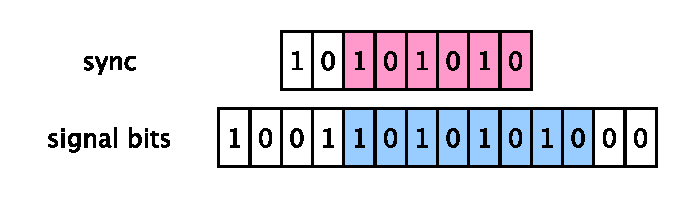
\includegraphics[width=0.45\textwidth]{figures/figure-sync-code-detection.pdf}
	\caption{\texttt{sync} Erkennung}
	\label{fig:sync-code-detection}
\end{wrapfigure}

Abbildung \ref{fig:sync-code-detection} skizziert das Erkennen eines Synchronisations-Codes \texttt{sync}\index{Synchronisations-Code}. Der Code wird immer mit einem Block Bits gleicher \mbox{Länge} des extrahierten Bitstroms verglichen. Die in der Skizze blau hervorgehobenen Bits sind das ein\-gebettete \texttt{sync}. Die rot markierten Bits signal\-isieren jene Zeichen, die beim \mbox{aktuellen} Vergleich über\-einstimmen. In diesem Beispiel beträgt die Über\-einstimmung zwischen er\-kanntem und tatsächlichem \texttt{sync} 75\% bei einer Synchronisation-Code Wortlänge von 8 Bit. Würde der Erkennungsschwellwert (oder \textit{Synccode-Threshold}\index{Synccode-Threshold}) ${T}_{s}$ 0.75 betragen, so wäre nun \texttt{sync} erkannt worden. Aus der Skizze ist aber ersichtlich, dass hier der tatsächlich Match erst 2 Shifts später erfolgt. Die anschließend gelesenen Informationsbits würden also teilweise aus dem Ende von \texttt{sync}\index{Synchronisations-Code} bestehen. Umgekehrt würden auch 2 echte Bits des Informationsblock\index{Information Block} nicht gelesen werden.

Das Problem in diesem Beispiel ist, dass \texttt{sync}\index{Synchronisations-Code} eine sehr hohe \textit{Autokorrelation}\index{Autokorrelation} besitzt. In anderen Worten ist \texttt{sync} (als Signal aufgefasst) sehr ähnlich zu sich selbst, weswegen 75\% Überdeckung auch zu 75\% Übereinstimmung führen. Die Lösung ist für \texttt{sync}\index{Synchronisations-Code} ein Sequenz mit minimaler Autokorrelation zu wählen. In der Literatur\cite{chang2012location}\cite{lie2006robust}\cite{huang2002blind} erfreuen sich die sog. \textit{Barker-Codes}\cite{barker1953group} großer Beliebtheit. Dabei handelt es sich um 9 Zahlensequenzen von denen der längste 13 Zeichen umfasst, welche alle die Bedingung der Autokorrelations-Funktion:

	 \begin{equation}
		 | \sum\limits_{j=1}^{N-v} a_j {a}_{j+} | \leq 1 \quad\mbox{mit}\quad 1 \leq v < N \quad\mbox{und}\quad a_j \in {-1,+1}
	 	\label{equ:barker-correlation}
	 \end{equation}

wobei $N$ die Code Länge bezeichnet, erfüllen. Es lässt sich zeigen, dass die Summe bei einer Verschiebung wie im Beispiel oben immer sehr klein ist, außer die Codes überdecken sich exakt. Gleichzeitig bleibt die Summe immer noch sehr groß (nahe an 1) wenn bei vollständiger Überdeckung innerhalb des Codes eine Zahl kippt. Ein gekipptes Bit wirkt sich also nicht so massiv auf die Erkennung des Codes aus wie eine falsche Überdeckung. Barker-Codes eignen sich daher hervorragend als Synchronisations-Code Sequenz. 

Die Länge der verwendeten Barker Sequenz wirkt sich natürlich auch auf die Erkennungsgenauigkeit aus. Hier wird der längste Barker-Code \textsf{+1 +1 +1 +1 +1 -1 -1 +1 -1 -1 +1 -1 +1} verwendet. Der Vollständigkeit halber sei noch darauf hingewiesen, dass wir nur Binärwerte kodieren können, weswegen $-1$ auf den Wert $0$ abgebildet wird. Bei der Erkennung von \texttt{sync} muss dies natürlich entsprechend bedacht werden.

Synchronisations-Codes werden genau wie die eigentlichen Informationen (die \textit{Nutzlast}) übertragen. Jeder eingebrachte \texttt{sync}\index{Synchronisations-Code} belastet daher die Transportkapazität des Signals. Es können also abhängig von der Informationsblocklänge bedeutend weniger Informationsbits effektiv in einem fixen Zeitfenster transportiert werden. 

\index{Barker-Code|)}
\index{Synchronisations-Code|)}

\subsection{Fehlerkorrekturverfahren} 
\label{sec:errorcorrection}
\index{Fehlerkorrekturverfahren|(}

Die Natur der Barker-Codes\index{Barker-Code} bringt eine gewisse Resistenz gegen Bitfehler mit sich, wie eben demonstriert wurde. Die Informationsbit haben diese im Allgemeinen nicht. Der Übertragungskanal\index{\"Ubertragungskanal} kann aber das Signal so weit beeinflussen, dass nicht alle Bits korrekt rekonstruiert werden. Es ist daher wünschenswert eine Methode zu verwenden welche derartige Bitfehler nicht nur erkennt, sondern auch korrigieren kann. Mit derartigen Modellen beschäftigt sich die \textit{Kodierungstheorie}\index{Kodierungstheorie}.

Wir verwenden hier eine Vorwärtsfehlerkorrektur\index{Vorwärtsfehlerkorrektur} (in der englischen Literator \textit{forward error correction}, daher kurz FEC) bei dem die Daten mit einem \textit{error-correcting code} \index{error-correcting code} (ECC\index{error-correcting code}) bewusst mit redundanten Daten angereichert werden. Aus dieser Redundanz lässt sich anschließend prüfen ob die Daten richtig rekonstruiert wurden und bei nicht zu starker Fehlerrate die tatsächliche Information auch wieder herstellen. 

In der Kodierungstheorie bezeichnet man mit \textit{Message}\index{Message} die Information die es zu übertragen gilt und mit \textit{Codeword}\index{Codeword} die mit Redundanz angereicherte Message. Im Informationsblock\index{\index{Information Block}} der einem jeden Synchronisations-Code\index{Synchronisations-Code} folgt befindet sich daher immer ein vollständiges Codeword um hier ggf. Übertragungsfehler auszugleichen. 

Bezeichnen wir mit $wmk$ das zu übertragende Watermark und mit ${L}_{w}$ seine Länge (sog. \textit{Watermark-Length}\index{Watermark-Length}, die Anzahl an Bit) dieses Watermarks, wobei $wmk(i)$ das Bit an der Stelle $i$ mit $i\in[1,{L}_{w}]$ referenziert, so ergeben sich folgende Bedingungen. Für die Bit-L\"ange einer Message ${L}_{m}$, genannt \textit{Message-Length}\index{Message-Length}, muss gelten:

	 \begin{equation}
		 {L}_{w} \pmod{{L}_{m}} = 0 \quad\mbox{und}\quad {L}_{w}\geq{L}_{m} 		
		 \label{equ:wmkseqlength}
	 \end{equation} 

und für die Bit-Länge eines Codewords ${L}_{c}$ (sog. \textit{Codeword-Length}\index{Codeword-Length}) gilt allgemein ${L}_{c} > {L}_{m}$
\\
Gültige Parameter für ${L}_{m}$ und ${L}_{c}$ hängen vom jeweiligen Fehlerkorrekturverfahren\index{Fehlerkorrekturverfahren} ab. Die im Folgenden angeführten Verfahren werden unterstützt:

\subsubsection{BCH-Codes}
\index{BCH-Codes}

In der Literatur\cite{chang2012location}\cite{huang2002blind} oftmals verwendet werden die nach Bose, Chaudhuri und Hocquenghem benannten BCH-Codes\cite{bose1960class}. Dabei handelt es sich um eine Gruppe von zyklischen Blockcodes um mehrere 1 Bit Fehler zu korrigieren. Es existieren verschiedene Codes und Implementierungen. Verwendet werden die System Objects \textsf{comm.BCHEncoder} und \textsf{comm.BCHDecoder} aus der MATLAB Communication System Toolbox.\footnote{\url{http://www.mathworks.de/de/help/comm/bch-codes.html}}.

\subsubsection{RS-Codes} 
\index{RS-Codes}

Reed-Solomon-Codes\cite{reed1960polynomial} (nach Irving S. Reed und Gustave Solomon) sind ebenfalls zyklischen Blockcodes, da sie eine Unterklasse der BCH-Codes sind. Ihr Prinzip ist einfach: Für eine Message\index{Message} aus $k$ Zeichen werden die $k$ Werte als Stützstellen eines Polynoms interpretiert. Mittels der Lagrange-Interpolation werden zusätzliche Stützstellen extrapoliert, sodass sich das Polynom durch $n>k$ Werte beschreiben lässt. Die $n$ Zeichen sind somit die Werte des Codewortes\index{Codeword}.

Bekannt wurden RS-Codes durch ihre Verwendung im Kommunikationsprotokoll der Voyager Sonden\footnote{Zwei interstellare Raumsonden der NASA, gestartet 1977. Beide sind heute noch aktiv (Stand 2014). Voyager 1 ist das am weitesten von der Erde entfernte, von Menschen gebaute Objekt.} und später als ECC-Verfahren\index{error-correcting code} bei CDs, DVDs, DSL oder DVB. 

Verwendet wird die MATLAB Implementierung der Communication System Toolbox\footnote{\url{http://www.mathworks.de/de/help/comm/reed-solomon-codes.html}}.

\subsubsection{LDPC-Codes}
\index{LDPC-Codes}

Low-Density-Parity-Check-Codes, von  Robert G. Gallager\cite{gallager1962low} entwickelt (daher oft auch Gallager-Codes), sind lineare ECC\index{error-correcting code} die nahe am Shannon-Limit (theoretische Obergrenze der Bitrate eines Übertragungskanals\index{\"Ubertragungskanal}) operieren. Sie sind daher ähnlich effektiv wie Turbo-Codes. Verwendung finden sie vor allem in der Fehlerkorrektur in WLAN-Standards.
Verwendet wird die MATLAB Implementierung der Communication System Toolbox\footnote{\url{http://www.mathworks.de/de/help/comm/ldpc-codes.html}}.

\index{Fehlerkorrekturverfahren|)}

\subsection{Datenstrukturen und Protokoll}
\label{sec:protokoll}
\index{Protokoll}

Jeder digitale Kommunikationsprozess basiert auf einem Protokoll welches alle Teilnehmer beherrschen müssen. So auch dieser hier, denn wenn gleich der Übertragungskanal auch analog sein mag, so werden doch digitale Daten übermittelt. Nicht nur gewährleistet ein definiertes Protokoll die korrekte Verarbeitung - die Abstrahierung erlaubt auch ein einfacheres Verständnis von Aufbau, Funktion und Zusammenspiel der einzelnen Teile. 

\begin{figure}[h]
	\centering
	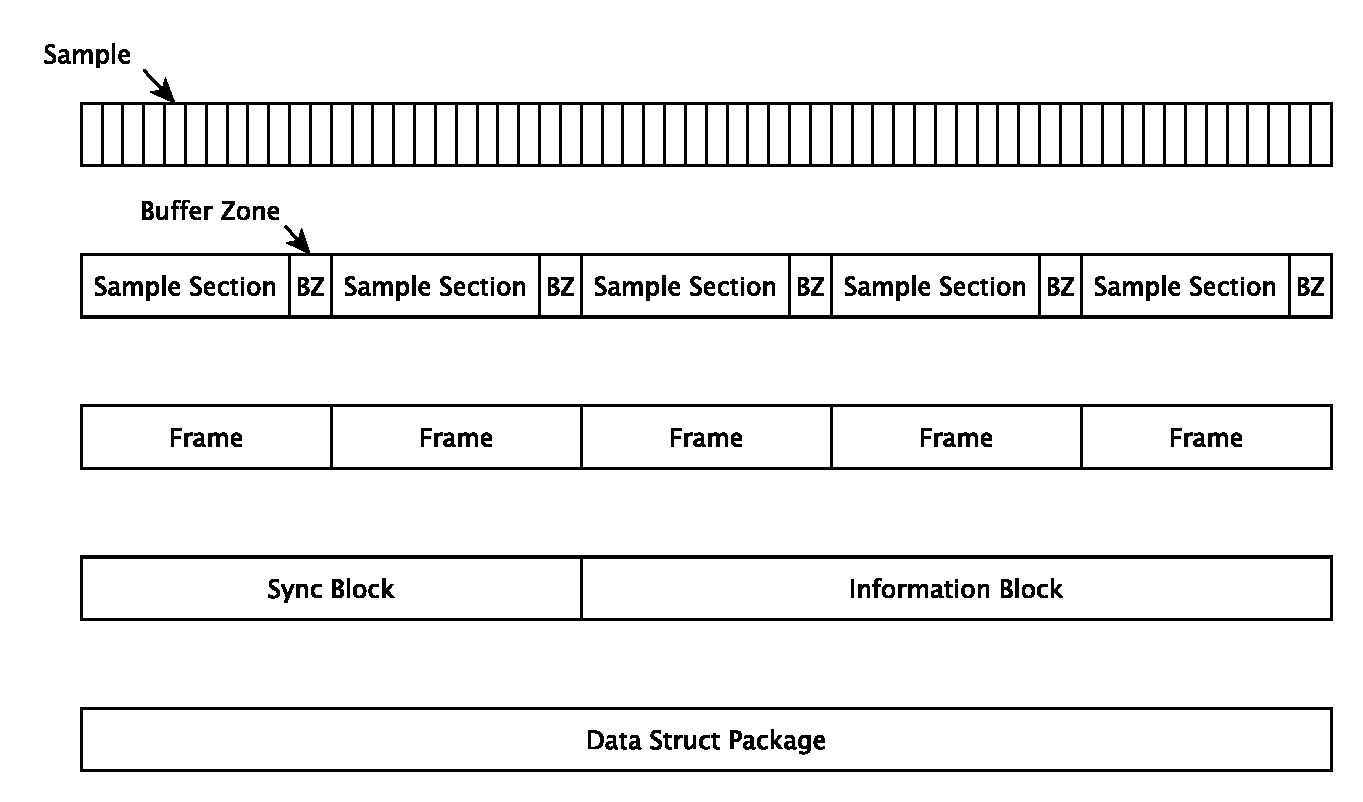
\includegraphics[width=\textwidth]{figures/figures-protocol.pdf}
	\caption{Hierarchischer Aufbau des Protokolls}
	\label{fig:protocol}
\end{figure}

\subsubsection{Sample Section}

Zunächst wird das Signal, welches durch zeit- und wertediskrete Samplewerten\index{Sample} beschrieben wird in Bereiche segmentiert. Es werden jeweils $N_s$\index{Sample-Section-Length} Samples\index{Sample} benötigt um 1 Bit zu transportieren. Dementsprechend werden genau die benötigte Anzahl aufeinanderfolgender Samples zu einer \textit{Sample Section} gruppiert.  

\subsubsection{Buffer Zones}
\index{Buffer Zones}

Um Interferenz zwischen den einzelnen Sample Sections\index{Sample Section} zu vermeiden befinden sich zwischen ihnen sog. \textit{Buffer Zones}. Dabei handelt es sich um eine an sich beliebige Anzahl an Samples\index{Sample}, die aber nicht zur Informationsübertragung verwendet werden. Bei der Verarbeitung der Samples werden die Buffer Zones einfach übersprungen. Prinzipiell können die Pufferzonen auch mit Sampleanzahl ${N}_{BZ} = 0$ definiert werden, allerdings führen Umweltfaktoren wie die Sensitivität des Aufnahmegerätes (und anderer AD Einflüsse \index{AD-Wandlung}) dazu, dass sich die Sample Sections überlagern\cite{chang2012location}. Das Ergebnis ist sog. \textit{Inter-Symbol-Interferenz}\footnote{Ein Symbol ist ein Element aus einem Alphabet. In binären Systemen ist das Alphabet also die Menge $\{0,1\}$.}. Die Auswirkung ist u.a. ein schlechteres Matching der Barker-Codes\index{Barker-Code} bei der Synchronisations-Code Erkennung\index{Synchronisations-Code}.

\subsubsection{Frame}
\index{Frame}

Um die Buffer Zones einfacher handzuhaben werden sie in den \textit{Frames} wegabstrahiert. Alle höheren Schichten sehen ein Frame als die logische Einheit die ein Bit transportiert. Einzig und allein die Frameverarbeitung muss über Position und Länge der Pufferzonen bescheid wissen. Für die höhere Schichten ist ein Bit in den ${N}_{F}$ Samples eines Frames, mit ${N}_{F} = {N}_{s} + {N}_{BZ}$, kodiert.

\subsubsection{Sync Block}
\index{Sync Block}

Ein Synchronisations-Code\index{Synchronisations-Code} besteht aus $L_s$\index{Synchronisations-Code-Length} Bit, daher sind ebenso viele Frames notwendig um ein \texttt{sync} zu schreiben. Diese Gruppe an Frames wird als \textit{Sync Block} bezeichnet.

\subsubsection{Information Block}
\index{Information Block}
 
Synchronisations-Codes\index{Synchronisations-Code} markieren die Stellen an denen Information vorhanden ist. Demensprechend ist jeder Sync-Block gefolgt von einem \textit{Information Block}, der sich aus $L_c$\index{Codeword-Length} aufeinander folgender Frames zusammensetzt. Ein Block transportiert immer ein vollständiges Codeword\index{Codeword}, beinhaltet somit also eine Message\index{Message} inklusive der Redundanz des ECC\index{error-correcting code}.

\subsubsection{Package}
\index{Package}

Ein Sync Block und sein Information Block bilden zusammen eine Einheit, sie existieren nie für sich alleine ohne den anderen. Demensprechend empfiehlt es sich sie in einer gemeinsamen Datenstruktur abzubilden, dem sog. \textit{Package}. Dieses eignet sich für die praktische Verwendung und lässt sich wie folgt Abbilden:


\lstset{escapechar=@,style=customc}         
\begin{lstlisting}
typedef enum { zero, one } bit_t;
typedef struct package {
    bit_t *header;
    bit_t *payload; 
} package_t;
\end{lstlisting}

Viele paketbasierte Netzwerkprotokolle definieren einen \textit{Header} (der das Packet beschreibt) und eine \textit{Payload} (die \glqq{}Nutzlast\grqq{}). Diesem entspricht auch ein Data Struct Package wenn man den Sync Block\index{Sync Block} als Header (auch wenn er nur angibt das es sich überhaupt um ein Packet handelt) und den Information Block\index{Information Block} als Payload auffasst.

Somit lässt sich der Übermittelungsprozess eines Watermarks\index{Watermark} konzeptionell beschreiben als eine Partitionierung des Watermarks in Messages geeigneter Länge (bedingt durch das Verhältnis $L_m$\index{Message-Length} zu $L_c$\index{Codeword-Length} des ECC\index{error-correcting code}) und deren Versand durch Pakete.

\subsubsection{Parallelen zum OSI-Modell}

Vergleicht man dieses Protokoll mit dem OSI-Modell\index{OSI-Modell}\footnote{\textit{Open Systems Interconnection Model}, auch ISO-OSI-Modell. Ein Netzwerkprotokolle mit Schichtenarchitektur. Früher tatsächlich in Verwendung, wird heute vor allem als Referenzmodell herangezogen.} so erkennt man folgendes: Frames\index{Frame} (und somit auch Sample Sections und Buffer Zones) sind hier Teil des \textit{Physical Layer} (Schicht 1), welcher sich um die Bitübertragung kümmert. Packages und deren Sync bzw. Information Blocks kümmern sich um  die Segmentierung von Bitdatenströmen in Blöcke und die Kanalkodierung. Sie bilden daher den \textit{Data Link Layer} (Schicht 2) ab.
 
\subsection{Qualitätskontrolle}
\label{sec:qualitaetskontrolle}
\index{Qualitätskontrolle|(}

Das Einbringen des Watermarks\index{Watermark} unterlieg der Bedingung, dass es unhörbar (für den Menschen) sein soll. Um dies zu gewährleisten muss jedes bearbeitete Teilstück des Signals einer Qualitätskontrolle diesbezüglich unterzogen werden. Dazu existieren prinzipiell folgende Methoden:

\subsubsection{Mean Opinion Score (MOS)}
\index{Mean Opinion Score}

Definiert in der ITU-T Recommendation P.800\cite{rec1996p} handelt es sich beim MOS um das Ergebnis der Bewertungen einer Reihe von subjektiven Wahrnehmungstest durch Versuchspersonen. Damit werden die Qualitäten von Codecs in der Sprach- und Bildübertragung bewertet. Da hierfür jedes Segment einzeln von menschlichen Versuchspersonen als Teil des Algorithmus behandelt werden müsste, eignet es sich ganz offensichtlich nicht eine automatische Verarbeitung. 

\subsubsection{Signal-Rauschabstand (SNR)} 
\index{Signal-Rauschabstand}

Der Signal-Rauschabstand oder Signal-Rausch-Verhältnis (engl. \textit{signal-to-noise ratio}, daher kurz SNR) bewertet die technische Qualität eines Signals welches von einem Störsignal überlagert wird. Hier ist zu beachten, dass mit Störsignal nicht jenes im analogen Übertragungskanal\index{\"Ubertragungskanal} gemeint ist. Die Veränderung eines Audiosignals durch das Watermark\index{Watermark} kann bezogen auf das ursprünglich unmodifizierte Signal ebenfalls als Störsignal interpretiert werden. 

Der SNR berechnet sich durch: 
	\begin{equation}	
		\mbox{SNR} = {\mbox{Nutzsignalleistung} \over \mbox{Rauschsignalleistung}},
		\label{equ:snr}
	\end{equation}

seine Bestimmung ist daher sehr einfach. Leider handelt es sich dabei um eine technisch objektive Güteeigenschaft die das menschliche Hörsystem nicht mit einbezieht und daher als Bewertungskriterium dementsprechend schlecht geeignet ist\cite{xiang2007robust}.

\subsubsection{Objective Difference Grade (ODG)} 
\index{Objective Difference Grade}
\index{Perceptual Evaluation of Audio Quality}

Offensichtlich ist es als notwendig ein automatisch berechenbares Qualitätskriterium heranzuziehen, welches allerdings eine auf die menschliche Wahrnehmung skalierte Bewertungsmetrik abbildet. Genau hierfür wurde 1998 die ITU Recommendation BS.1387\cite{rec1998bs}, besser bekannt als \textit{Perceptual Evaluation of Audio Quality} (PEAQ) spezifiziert. Mit ihr lässt sich für ein Audiosignal der sog. \textit{Objective Difference Grade} (ODG) berechnen, ein Wert im Intervall $[-4,0]$ wobei $0$ für  \glqq{}unhörbar\grqq{} und $-4$ für \glqq{}sehr störend\grqq{} steht. Es hat sich gezeigt, dass die Korrelation von PEAQ Bewertung und MOS ca. 0.98 beträgt\cite{al2011dwt}.

Leider hat sich recht bald herausgestellt, dass die Berechnung des ODGs nicht hinreichend genau spezifiziert ist\cite{kabal2002examination}\cite{campeanu2005peaq}, was sich auch in der Qualität der derzeit vorhandenen Tools wiederspiegelt. Eine kurze Evaluierung gängiger PEAQ Implementierungen findet sich in Anhang \ref{ch:peaq}.

\index{Qualitätskontrolle|)}

\newpage

\section{Watermark Extrahierung}
\label{sec:extraction}

Nachdem das Watermark\index{Watermark} nach den nun beschriebenen Schritten in ein Signal eingebettet und anschließend übertragen wurde, gilt es nun die Informationsdaten wieder zu extrahieren. Abbildung \ref{fig:diagram-decoder} zeigt den schematischen Ablauf des Dekodierungsprozesses.

\begin{figure}[h]
	\centering
	%\includesvg[width=0.7\textwidth]{figures/diagram-framework.svg}
	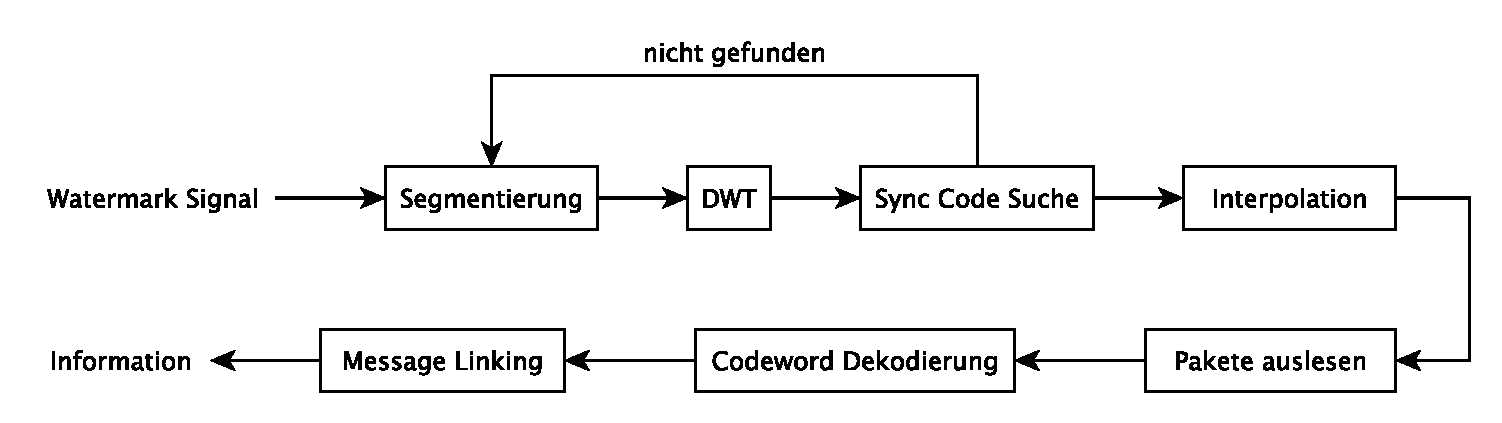
\includegraphics[width=0.9\textwidth]{figures/diagram-decoder-v2.pdf}
	\caption{Schematischer Aufbau des Extraktionsprozesses}
	\label{fig:diagram-decoder}
\end{figure}


\subsection{Resynchronisaton und Interpolation}

Bei der Erkennung der Synchronisations-Codes kann es im Allgemeinen zu Problemen kommen. Die bei der DA-Wandlung\index{DA-Wandlung} auftretenden Einflüssen lassen sich im Allgemeinen durch eine Kombination aus \textit{time scaling modification}\index{time scaling modification} (kurz TSM, dt. interessanterweise bekannt als \textit{Time-Stretching}) und \textit{wave magnitude
distortion}\textit{wave magnitude
distortion} (WMD) beschreiben\cite{xiang2007robust}\cite{steinebach2002audio}. Die TSM kann das Auffinden der Synchronisation-Codes verhindern. Das Prinzip kann daher auch gezielt eingesetzt werden, um ein existierendes Watermark\index{Watermark} zu zerstören (etwa um einen Urheberrechtlichsschutz aufzuheben). Dies wird als \textit{Synchronization attack}\index{Synchronization attack} bezeichnet.

Um diesen Effekt der DA-Wandlung\index{DA-Wandlung} aufzuheben, muss versucht werden die Synchron\-isations\--Codes wieder\-herzustellen. Man nennt diesen Vorgang \textit{Resynchronisation}\index{Resynchronisation}. Verschiedene Resynchronisationsansätze existieren, hier wird ein sog. \textit{brute-force approach}\index{brute-force approach} angewandt und wie in \cite{steinebach2011re} vorgeschlagen auf ein Suchintervall von -10\% bis +10\% beschränkt. 

Die TSM bewirkt, dass das Signal auf seiner Zeitachse gestreckt oder gestaucht wird. Für das Watermark\index{Watermark} bedeutet das, dass ein Bit nicht mehr in $N_s$\index{Sample-Section-Length} Samples kodiert ist, sondern durch mehr oder weniger Samples ${N}_{s}'$ beschrieben wird. 
Zuerst gilt es die neue Sampleanzahl ${N}_{s}'$ zu finden. Dazu wird ${N}_{s}'$ von $0.9 \cdot {N}_{s}$ bis $1.1 \cdot {N}_{s}$ durchgetestet und nach Synchronisations-Codes\index{Synchronisations-Code} gesucht. Algorithmus \ref{alg:resync} illustriert diesen Vorgang.

\RestyleAlgo{algoruled}
\begin{algorithm}[h]

	\SetKwData{Framelen}{framelen}
	\SetKwData{Ns}{${N}_{s}$}
	\SetKwData{Steplen}{steplen}
	\SetKwData{Upperbound}{upperbound}
	\SetKwData{Lowerbound}{lowerbound}
	\SetKwData{Sig}{sig}
	\SetKwData{Size}{size}
	\SetKwData{Testwindow}{testwindow}
	\SetKwData{Cursor}{cursor}
	\SetKwData{Found}{found}
	\SetKwFunction{Resynchronize}{resynchronize}
	\SetKwFunction{Testsync}{testsync}
	\SetKwInOut{Input}{input}
	\SetKwInOut{Output}{output}

\Input{Samples eines Signals}
\Output{Resynchronisiertes Signal}

\BlankLine

\Steplen = 0.005 * \Ns\;
\Lowerbound = 0.9 * \Ns\;
\Upperbound = 1.1 * \Ns\;
\Cursor = 1\;

\While{ \Cursor < \Size - \Upperbound and not \Found }{
	\Framelen = \Lowerbound\;
	\While{\Framelen < \Upperbound}{
		\Testwindow = \Sig[\Cursor,\Framelen]\;
		\Found = \Testsync{\Testwindow}\;
		\eIf{\Found}{ 
			\Resynchronize{\Sig,\Framelen}\;
		}{ 
			\Framelen = \Framelen + \Steplen\;
		}
	}
	\Cursor = \Cursor + 0.1 * \Lowerbound\; 
}
\caption{\texttt{sync} Erkennung in der Resynchronisationsphase}
\label{alg:resync}
\end{algorithm}


Wurde ein \texttt{sync}\index{Synchronisations-Code} gefunden, so kann man das Verhältnis zwischen neuer und alter Sampleanzahl

	\begin{equation}
		\alpha = { {N}_{s}' \over {N}_{s} }
		\label{equ:resampling_factor}
	\end{equation}
	\index{Sample-Section-Length}

berechnet werden. Mit $\alpha$ können nun alle Samples als Vorverarbeitungsschritt auf ihren ursprünglichen Wert rückinterpoliert werden. Verschiedene Interpolationsverfahren führen hier zu keinem merklichen Unterschied\cite{xiang2007robust}, weswegen eine lineare Lagrange-Interpolation\index{Lagrange-Interpolation} verwendet wird. Somit können die neuen Samplewerte $f''(i)$ durch

	\begin{equation}
		f''(i) = \begin{cases}
    	 	f'(i) & \iff i = 1	
			\\
			(1-\beta) \cdot f'(\lfloor\alpha \cdot i\rfloor) + \beta \cdot f'(\lfloor\alpha \cdot i\rfloor + 1) & \iff 1 < i < {N}_{s} 
			\\
    		f({N}_{s}') & \iff i = {N}_{s}
  		 \end{cases}
		\label{equ:lagrange_interpolation}
	\end{equation}
	
wobei $f'(i)$ die alten Werte und $\beta = \alpha \cdot i - \lfloor \alpha \cdot i \rfloor$ beschreibt, berechnet werden. Somit kann für die Extrahierung das exakt selbe Verfahren zur Analyse der DWT-Koeffizienten\index{DWT-Koeffizienten} wie im Implantationsprozess verwendet werden. 

\subsection{Datenextrahierung}

Nach der Resynchronisation kann das Signal schrittweise durchlaufen und nach \texttt{sync} Sequenzen gescannt werden. Dabei wird das Signal genau so wie in der Implementierungsphase in Samples Sections zerteilt, die DWT-Koeffizienten für die Samples berechnet und nach dem Prinzip aus Kapitel \ref{sec:reconstruction} für jedes Segment ein binärer Wert bestimmt. Anschließend werden immer $L_s$\index{Synchronisations-Code-Length} aufeinander folgende Binärwerte auf ihre Übereinstimmung mit dem Synchronisations-Code\index{Synchronisations-Code} \texttt{sync} überprüft.

Erfolgt ein Match auf den Synchronisations-Code, so sind die folgenden $L_c$\index{Codeword-Length} Bit als Informationsbits aufzufassen. Da es sich um ein Codeword\index{Codeword} handelt, muss noch der Dekodierungsalgorithmus des ECC\index{error-correcting code} angewendet werden, um die Message\index{Message} zu erhalten. Die einzelnen Messages ergeben schließlich zusammengesetzt die eigentliche Information. 

Wie man sich anhand der Abbildung \ref{fig:protocol} leicht überlegen kann, können immer nachdem ein Codeword erfolgreich gelesen wurde die folgenden $L_c$\index{Codeword-Length} Samples Sections \index{Sample Section} auf der Suche nach weiteren \texttt{sync}\index{Synchronisations-Code} Sequenzen übersprungen werden.





%%%%%%%%%%%%%%%%%%%%%%%%%%%%%%%%%%%%%%%%%
\chapter{Analyse}
\label{ch:analyse}



\section{Payload Performance}
\label{sec:payloadperformance}

\section{Stirmark Benchmarks}

Hierfür wird wohl Stirmark Benchmarks\cite{petitcolas2000watermarking}\cite{petitcolas2004stirmark} (\url{http://www.petitcolas.net/fabien/watermarking/stirmark/}) verwendet werden

\section{Manuelle Synchronisation}

Um die Ursachen für die scheiterne Übertragung im analogen Bereich zu analysieren wurden Signale manuell synchronisiert. Dies erlaubt die DWT-Koeffizientn\index{DWT-Koeffizienten} direkt mit dem ursprünglichen Signal zu vergleichen. Somit lassen sich die Ursachen ausfindig machen

+ Subband Engielevel

+ koeffizienten direkt

+ synchronisation

+ error correction

\section{Robustheit}

\subsection{MP3}

\subsection{Lautstärke}

\subsection{Rauschen}

\subsection{Übertragungskanäle}

\subsubsection{Digital}

\subsubsection{Analog}

\paragraph{Signalkabel}

\paragraph{Luft}







%%%%%%%%%%%%%%%%%%%%%%%%%%%%%%%%%%%%%%%%%
\chapter{Schlussfolgerung und Ausblick}
\label{ch:ausblick}

Im Zuge der Implementierung hat sich nach den ersten DA/AD-Tests sehr schnell gezeigt, dass die verwendete Watermarking Methode\cite{xiang2007robust} nicht das zu leisten vermag, was sie verspricht. Wenn gleich das Watermark\index{Watermark} im rein digitalen an der Hörschwelle stabil ist, so ist die Resistent im analogen Kanal unbefriedigend. Die daraufhin angebrachten Erweiterungen um Fehlerkorrekturverfahren\index{Fehlerkorrekturverfahren} haben auch hier nur eingeschränkt für Veresserung gesorgt. Das Problem scheint vor allem in der Anfälligkeit der Synchronisations-Codes\index{Synchronisations-Code} zu liegen. 

Allerdings sieht das entwickelte Framework als grundlegende Architektur dennoch sehr vielversprechend aus. Das sehr einfach definierte Protokoll\index{Protokoll} ist flexibel bezüglich der angewendeten Methoden seiner Komponenten. Es wäre daher ein leichtes die Watermarkung-Methode gegen eine sich als robuster erwießenere auszutauschen. Sehr vielversprechend erscheint hier etwa die Puplikation von Chang, Di, et al.\cite{chang2012location}. Somit könnte das Framework unverändert weiter benützt werden nachdem lediglich die Funktionen zum lesen und schreiben eines Bits angepasst werden würden. 

Weiters hat sich die Qualität der aktuell vefügbaren PEAQ-Implementierungen\index{Perceptual Evaluation of Audio Quality} als unzureichend erwießen. Zu viele Probleme und Ergebnisse die mit subjektiven Hörtests nicht bestätigt werden können lassen die Evaluierung des Watermarkingprozesses oftmals in unzureichendem Zustand. Eine mögliche Besserung könnte der PEAQ Konkurent PEMO-Q\cite{huber2006pemo} bringen. Über die Verfügbarkeit von Tools wurden im Zuge dieser Arbeit keine Informationen eingeholt. 

Wenig performant ist derzeit der Re\-synchron\-isations\-prozess. Die Suche nach Synchron\-isations-Codes wird derzeit über einen einfachen brute-force Ansatz gelöst. Dieser ist nicht nur langsam, sondern liefert im Allgemeinen auch eine nicht optimale Lösung. Hier würden sich die in \cite{steinebach2011re} angeführten Alternativen anbieten, sowie eine Lokale Suche um das Optimierungs\-problem zu verbessern. 

%%%%%%%%%%%%%%%%%%%%%%%%%%%%%%%%%%%%%%%%%



%%%%%%%%%%%%%%%%%%%%%%%%%%%%%%%%%%%%%%%%%
%%% BACKMATTER %%%%%%%%%%%%%%%%%%%%%%%%%%
%%%%%%%%%%%%%%%%%%%%%%%%%%%%%%%%%%%%%%%%%

\appendix

\begin{appendix}

%%%%%%%%%%%%%%%%%%%%%%%%%%%%%%%%%%%%%%%%%

\chapter{PEAQ Implementierungen}
\label{ch:peaq}

\section{EAQUAL}

\section{PQevalAudio}

\section{peaqb}

Bei \texttt{peaqb} handelt es sich um die Bemühung eine Implementation der Recommendation ITU-R BS.1387-1 als freie offene Software zu schaffen. Initiier im Jahr 2003 liegt seit dem 14. März 2013 das GPLv2 lizensierte Tool in der Version 1.0 Beta vor. Zu finden ist das Projekt auf der Softwareentwicklungsportal Sourceforge\footnote{\url{http://sourceforge.net/projects/peaqb/}}, welche sich nicht ganz unbegr\"undet in den letzten Jahre den inoffiziellen Beinahmen \glqq Friedhof der Open Source Projekte\grqq{} eingefangen hat, was auch bei peaq leider zu spühren ist. 

Die Versuche \texttt{peaqb} für die Signal-Qualitätssicherung zu bem\"uhen haben schnell gezeigt, dass das Tool noch sehr instabil ist. In den meisten F/"allen terminiert das Programm mit einem Segmentation Fault. Falls es in der Lage ist Endergebnisse zu berechnen, so sind diese oftmals ähnlich zu PQevalAudio unbrauchbar, da sie entweder ebenfalls in nicht definierten Bereichen liegen oder mit der subjektiven H\"orwahrnehmung einfach nicht \"ubereinstimmen. 

Eine Weiterentwicklung jenseits einer Version 1.0 Beta ist nicht abzusehen. 

\section{OPERA}






%%%%%%%%%%%%%%%%%%%%%%%%%%%%%%%%%%%%%%%%%




\end{appendix}

\bibliographystyle{plain}
\bibliography{references}

\end{document}
